\documentclass[12pt,a4paper]{article}
\usepackage{ctex}
\usepackage{amsmath,amscd,amsbsy,amssymb,latexsym,url,bm,amsthm}
\usepackage{epsfig,graphicx,subfigure}
\usepackage{enumitem,balance}
\usepackage{wrapfig}
\usepackage{mathrsfs,euscript}
\usepackage[usenames]{xcolor}
\usepackage{hyperref}
\usepackage[vlined,ruled,linesnumbered]{algorithm2e}
\hypersetup{colorlinks=true,linkcolor=black}

\newtheorem{theorem}{Theorem}
\newtheorem{lemma}[theorem]{Lemma}
\newtheorem{proposition}[theorem]{Proposition}
\newtheorem{corollary}[theorem]{Corollary}
\newtheorem{exercise}{Exercise}
\newtheorem*{solution}{Solution}
\newtheorem{definition}{Definition}
\theoremstyle{definition}

\renewcommand{\thefootnote}{\fnsymbol{footnote}}

\newcommand{\postscript}[2]
 {\setlength{\epsfxsize}{#2\hsize}
  \centerline{\epsfbox{#1}}}

\renewcommand{\baselinestretch}{1.0}

\setlength{\oddsidemargin}{-0.365in}
\setlength{\evensidemargin}{-0.365in}
\setlength{\topmargin}{-0.3in}
\setlength{\headheight}{0in}
\setlength{\headsep}{0in}
\setlength{\textheight}{10.1in}
\setlength{\textwidth}{7in}
\makeatletter \renewenvironment{proof}[1][Proof] {\par\pushQED{\qed}\normalfont\topsep6\p@\@plus6\p@\relax\trivlist\item[\hskip\labelsep\bfseries#1\@addpunct{.}]\ignorespaces}{\popQED\endtrivlist\@endpefalse} \makeatother
\makeatletter
\renewenvironment{solution}[1][Solution] {\par\pushQED{\qed}\normalfont\topsep6\p@\@plus6\p@\relax\trivlist\item[\hskip\labelsep\bfseries#1\@addpunct{.}]\ignorespaces}{\popQED\endtrivlist\@endpefalse} \makeatother

\begin{document}

\noindent

%========================================================================
\noindent\framebox[\linewidth]{\shortstack[c]{
\Large{\textbf{Lab08-Graph Exploration}}\vspace{1mm}\\
CS214-Algorithm and Complexity, Xiaofeng Gao, Spring 2020.}}
\begin{center}
\footnotesize{\color{red}$*$ If there is any problem, please contact TA Yiming Liu.}

\footnotesize{\color{blue}$*$ Name:Hongjie Fang  \quad Student ID:518030910150 \quad Email: galaxies@sjtu.edu.cn}
\end{center}

\begin{enumerate}
    \item
    \textbf{BFS Tree.} Similar to DFS, BFS yields a tree, (also possibly forest, but \textbf{just consider a tree} in this question) and we can define \textbf{tree, forward, back, cross} edges for BFS. Denote $Dist(u)$ as the distance between node $u$ and the source node in the BFS tree. Please prove:
    \begin{enumerate}
    	\item For both undirected and directed graphs, no forward edges exist in the graph.
    	
    	\item There are no back edges in undirected graph, while in directed graph each back edge $(u,v)$ yields $0\leq Dist(v)\leq Dist(u)$.
    	
    	\item For undirected graph, each cross edge $(u,v)$ yields $|Dist(v)-Dist(u)|\le 1$, while for directed graph, each cross edge $(u,v)$ yields $Dist(v)\leq Dist(u)+1$.
    	
    \end{enumerate}

    \begin{proof} We have already learnt that $Dist(u)$ means \underline{the fewest number of edges} in a path from source to $u$ in the graph according to the BFS process. What's more, the $Dist$ value is exactly the depth of a node in BFS tree if we set the depth of the root to $0$, since the calculations of depth and $Dist$ are exactly the same. Here are the proofs for each sub-question.
    \begin{enumerate}
    \item
    \begin{itemize}
         \item \textbf{\color{purple} Directed graph case: }
         \textbf{(Contradiction)} Suppose there exists one forward edge $(u, v)$ in the directed graph. On one hand, according to the definition of the forward edge, $v$ is a non-child descendant of $u$, which indicates that the difference between the depth of $u$ and the depth of $v$ is at least $2$, that is,
         \begin{equation}
         Dist(v) - Dist(u) \geq 2
         \label{eq1}
         \end{equation}
         On the other hand, according to the definition of $Dist$, we can derive that
         \begin{equation}
         Dist(v) \leq Dist(u) + 1
         \label{eq2}
         \end{equation}
         because there is a path from source to $u$ using $Dist(u)$ edges and there is an edge from $u$ to $v$. It's easy to derive a contradiction when combining Equation \eqref{eq1} and Equation \eqref{eq2} together. Therefore, no forward edges exist in the directed graph.
         \item \textbf{\color{purple} Undirected graph case: } Using exactly the same method in the proof of the directed graph, we can prove the conclusion is still correct for undirected graph, that is, no forward edges exist in the undirected graph.
    \end{itemize}
    \item
        \begin{itemize}
        \item \textbf{\color{purple} Directed graph case: }
        We know that the $Dist$ value of node $u$ is basically the depth of $u$ in BFS tree. For every back edge $(u, v)$ in the directed graph, $v$ is the ancestor of $u$, which indicates that the depth of $v$ is less than the depth of $u$, that is, $Dist(v) \leq Dist(u)$. It is obvious that that all the $Dist$ values are non-negative, that is, $Dist(v) \geq 0$. Hence, in directed graph, each back edge $(u,v)$ yields:
        \begin{displaymath}
        0 \leq Dist(v) \leq Dist(u)
        \end{displaymath}
        \item \textbf{\color{purple} Undirected graph case: }
        \textbf{(Contradiction)} Every undirected back edge $(u, v)$ can be viewed as an undirected forward edge $(v, u)$ in undirected graph (the back edge to one's parent cannot exist because the edge is actually a tree edge), because they are actually the same edge represented in two different ways. Suppose there exists one back edge $(u, v)$ in the undirected graph, then a forward edge $(v, u)$ exists in the undirected graph, which contradicts the conclusion in the first sub-question. Therefore, there are no back edges in undirected graph.
        \end{itemize}
        \clearpage
    \item \begin{itemize}
    \item \textbf{\color{purple} Directed graph case: } \textbf{(Contradiction)} Suppose there is one cross edge $(u, v)$ satisfying $Dist(v) > Dist(u) + 1$ in the directed graph (Fig.~\ref{fig1-1}).
        \begin{figure}[h]
          \centering
          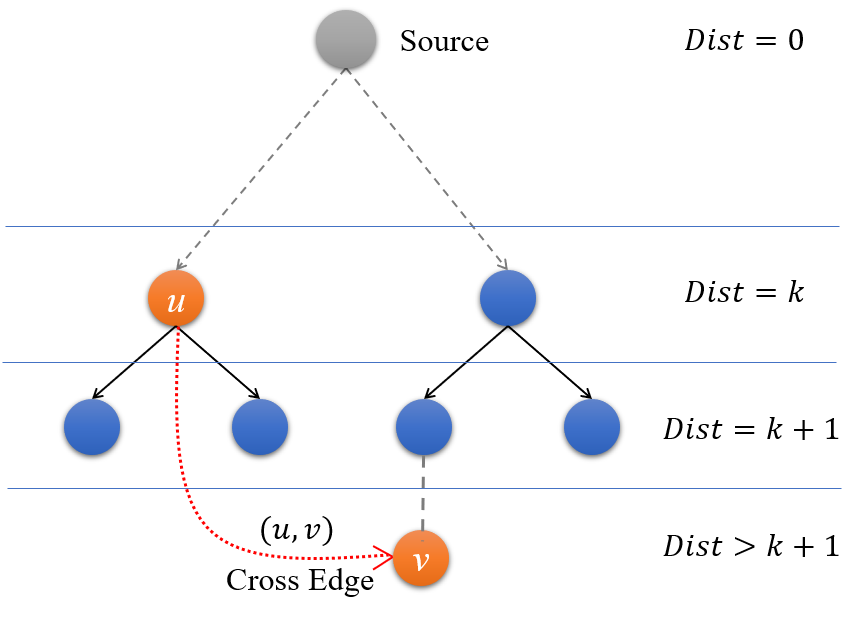
\includegraphics[width=4.5in]{figures/prob1-3.png}\\
          \caption{The situation in a directed graph}\label{fig1-1}
        \end{figure}

        According to the definition of $Dist$, we can derive that
        \begin{equation}
        Dist(v) \leq Dist(u) + 1
        \label{eq3}
        \end{equation}
        because there is a path from source to $u$ using $Dist(u)$ edges and there is an edge from $u$ to $v$. It's easy to find that Equation \eqref{eq3} contradicts our premise. Therefore, for directed graph, each cross edge $(u,v)$ yields $Dist(v)\leq Dist(u)+1$.
    \item \textbf{\color{purple} Unirected graph case: } \textbf{(Contradiction)} Suppose there is one cross edge $(u, v)$ satisfying $|Dist(v) - Dist(u)| > 1$ in the undirected graph.
        \begin{itemize}
        \item On one hand, if $Dist(v) - Dist(u) > 1$, we can use exactly the same method in the proof of directed graph to come to a contradiction.
        \item On the other hand, if $Dist(v) - Dist(u) < -1$, we can rewrite the inequality to $Dist(u) - Dist(v) > 1$, and we can use exactly the same method in the proof of directed graph, except changing the position of $u$ and $v$, to come to a contradiction.
        \end{itemize}
        Hence, both situation have contradictions. Therefore, for undirected graph, each cross edge $(u,v)$ yields $|Dist(v)-Dist(u)|\le 1$.
    \end{itemize}
    \end{enumerate}
    \end{proof}
    \clearpage


    \item
    \textbf{Articulation Points, Bridges, and Biconnected Components.} Let $G=(V, E)$ be a connected, undirected graph. An articulation point of $G$ is a vertex whose removal disconnects $G$. A bridge of $G$ is an edge whose removal disconnects $G$. A biconnected component of $G$ is a maximal set of edges such that any two edges in the set lie on a common simple cycle. Figure\ref{def} illustrates these definitions. We can determine articulation points, bridges, and biconnected components using depth-first search. Let $G_{\pi}=\left(V, E_{\pi}\right)$ be a depth-first tree of $G$. Please prove:

    \begin{enumerate}
    	\item The root of $G_{\pi}$ is an articulation point of $G$ if and only if it has at least two children in $G_{\pi}$.
    	\item An edge of $G$ is a bridge if and only if it does not lie on any simple cycle of $G$.
    	\item The biconnected components of $G$ partition the nonbridge edges of $G$.
    \end{enumerate}

	 \begin{figure}[htbp]
		\centering
		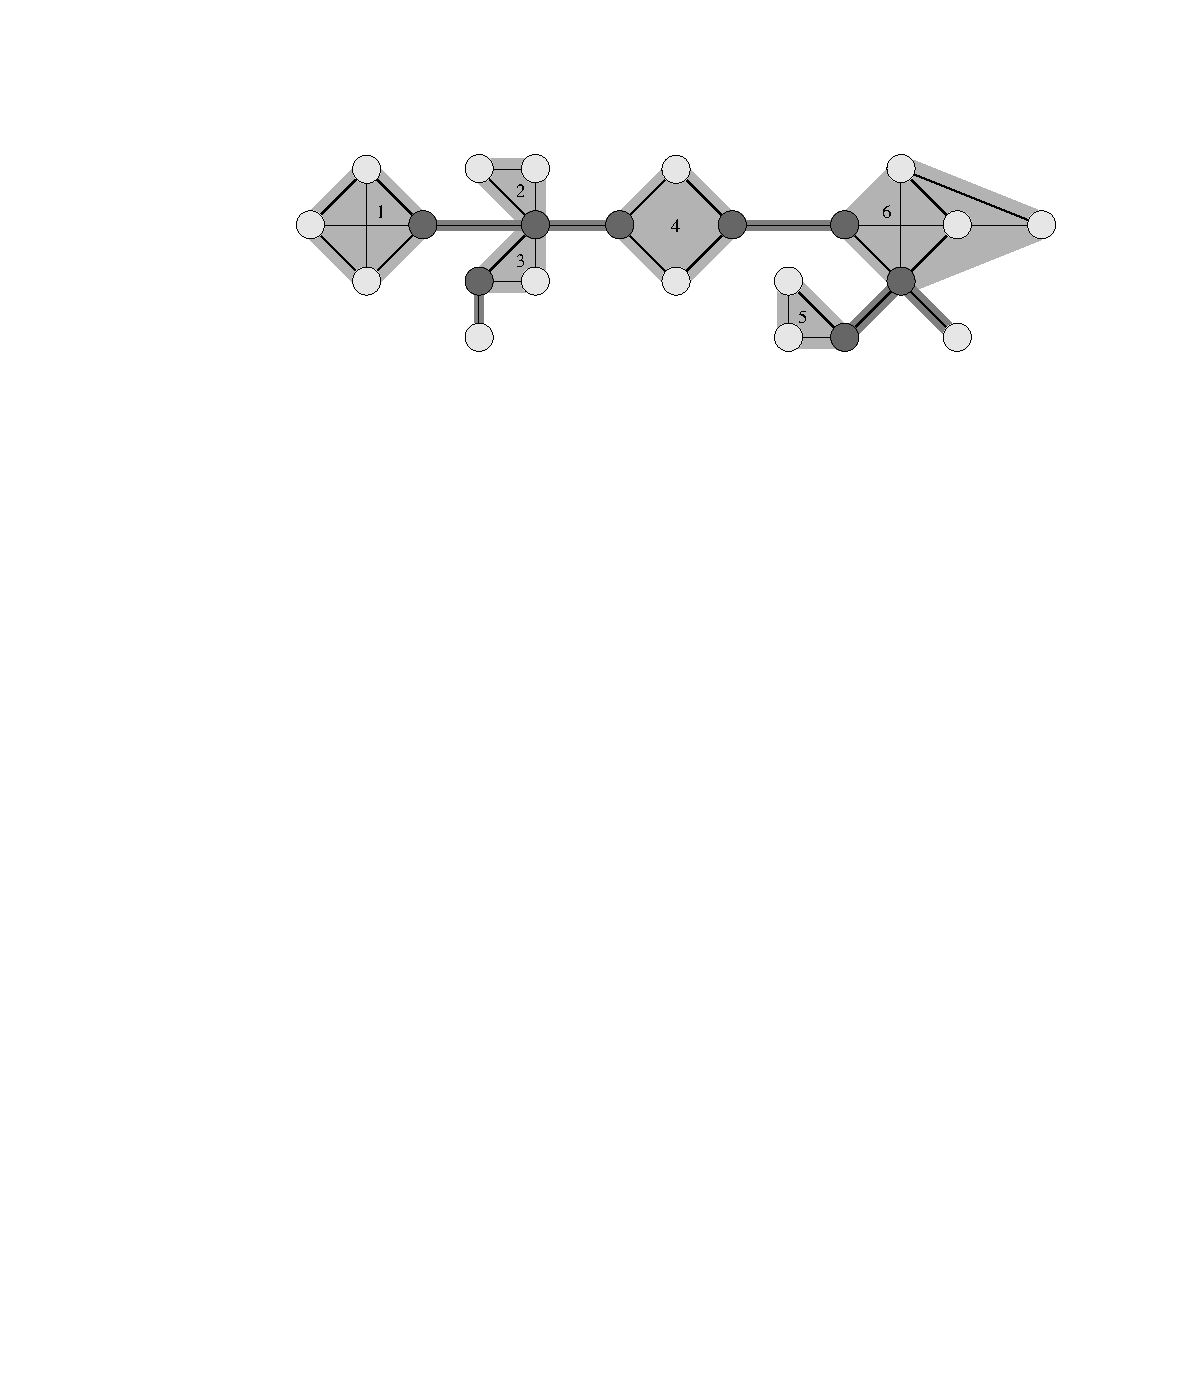
\includegraphics[width=6in]{Fig-Definition.pdf}
		\caption{The definition of articulation points, bridges, and biconnected components. The articulation points are the heavily shaded vertices, the bridges are the heavily shaded edges, and the biconnected components are the edges in the shaded regions, with a \textit{bcc} numbering shown.}
		\label{def}
	\end{figure}

    \begin{proof} Here are the proofs for each sub-question.
    \begin{enumerate}
    \item
        \begin{itemize}
        \item \textbf{($\Longleftarrow$)} Since the root has at least two children in $G_{\pi}$, we are able to choose two distinct children of root of $G_{\pi}$, say $c_1$ and $c_2$. According to the DFS algorithm and the DFS tree, there exists no path linking nodes in subtree $c_1$ and nodes in subtree $c_2$ in graph $G$ (Fig.~\ref{fig2-1}), or $c_1$ and $c_2$ should be in the same subtree in $G_{\pi}$ because we can visit $c_2$ starting from subtree $c_1$ without visiting root and vice versa. Thus, when removing root from $G$, two subtrees $c_1$ and $c_2$ are disconnected. Therefore, if the root has at least two children in $G_{\pi}$, then it is the articulation point.
            \begin{figure}[h]
              \centering
              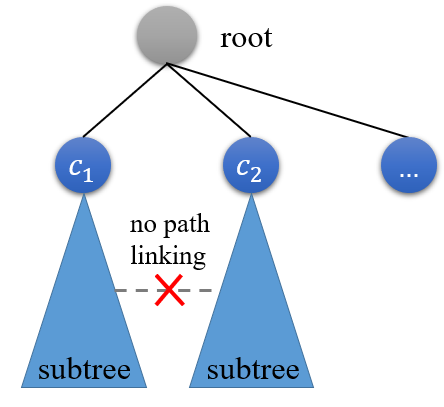
\includegraphics[width=2in]{figures/prob2-1-1.png}\\
              \caption{The situation when the root has at least two children in $G_{\pi}$}\label{fig2-1}
            \end{figure}
        \item \textbf{($\Longrightarrow$)} \textbf{(Contradiction)} Suppose the root has no more than one child in $G_{\pi}$. If the root has no children, which means it is a connected component itself, then it is obvious that the root is not a articulation according to the definition of articulation point, which contradicts the premise. Thus, the root must have only one child, say $c$. There are totally two situations when the root has only one child in $G_{\pi}$ (Fig. \ref{fig2-2}).
             \begin{figure}[h]
                \centering
                \subfigure[Situation a] {
                    \begin{minipage}[t]{0.4\linewidth}
                        \centering
                        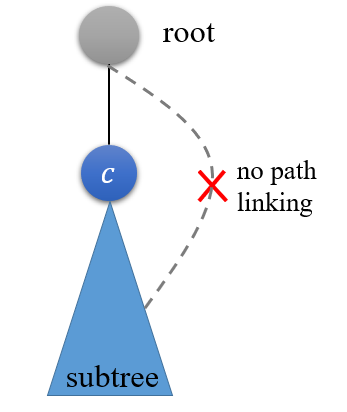
\includegraphics[width=1.6in]{figures/prob2-1-2a.png}
                    \end{minipage}
                    \label{fig2-2a}
                }
                \subfigure[Situation b] {
                    \begin{minipage}[t]{0.4\linewidth}
                        \centering
                        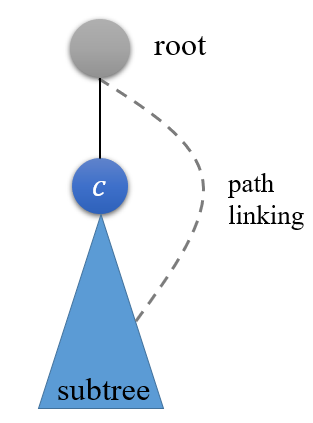
\includegraphics[width=1.6in]{figures/prob2-1-2b.png}
                    \end{minipage}
                    \label{fig2-2b}
                }
              \caption{The situations when the root has only one child in $G_{\pi}$}\label{fig2-2}
            \end{figure}
            \begin{itemize}
            \item \textbf{Situation a} (Fig. \ref{fig2-2a}) The subtree of $c$ does not have a path linking the subtree of $c$ and the root.
            \item \textbf{Situation b} (Fig. \ref{fig2-2b}) The subtree of $c$ has a path linking the subtree of $c$ and the root.
            \end{itemize}
            Whatever the situation is, if we remove root from $G$, the rest part of the graph is still connected. Hence, the root is not an articulation point, which contradicts the premise. Therefore, if the root of $G_{\pi}$ is an articulation point, then it has at least two children in $G_{\pi}$.
        \end{itemize}
    \item
        \begin{itemize}
        \item \textbf{($\Longleftarrow$)} Since an edge $e = (u, v)$ does not lie on any simple cycle, there exists no simple path linking $u$ and $v$ if we remove edge $e$ from $G$ (Fig.~\ref{fig2-3}). That's because if we have such path, then the simple path and edge $e$ will form a cycle in graph $G$, which contradicts the premise that $e$ does not lie on any simple cycle of $G$. Thus, if we remove edge $e$ from $G$, node $u$ and node $v$ will become disconnected because there is no path linking them in the rest part of $G$, which indicates $e$ is a bridge. Therefore, if an edge does not lie on any simple cycle of $G$, then it is a bridge.
            \begin{figure}[h]
              \centering
              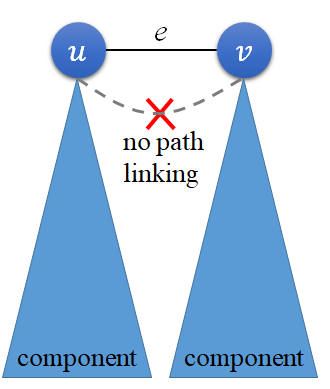
\includegraphics[width=1.6in]{figures/prob2-2-1.png}\\
              \caption{The situation when edge $e$ does not lie on any simple cycle in $G$}\label{fig2-3}
            \end{figure}
        \item \textbf{($\Longrightarrow$)} \textbf{(Contradiction)} Suppose edge $e = (u,v)$ lies on one simple cycle, then there must exist a simple path linking $u$ and $v$ without edge $e$ (Fig.~\ref{fig2-4}), say $P$, because path $P$ and edge $e$ will form a simple cycle. Then if we remove $e$ from graph $G$, the rest part of graph is still connected, because \underline{path $P$ can play the role of edge $e$} to link $u$ and $v$, that is, all paths that use edge $e$ can replace edge $e$ by path $P$ without changing the connectivity. Thus, all the connected nodes are still connected in the new graph without edge $e$, and it indicates that $e$ is not a bridge, which contradicts the premise. Therefore, if edge $e$ is a bridge, then it does not lie on any simple circle of $G$.
            \begin{figure}[h]
              \centering
              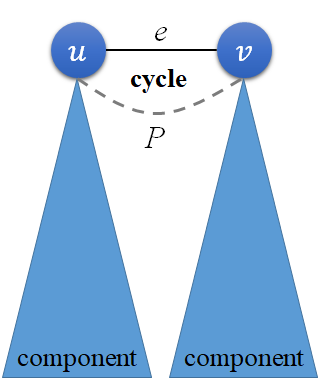
\includegraphics[width=1.5in]{figures/prob2-2-2.png}\\
              \caption{The situation when edge $e$ lies on one simple cycle in $G$}\label{fig2-4}
            \end{figure}
        \end{itemize}
    \item There are two main points that we try to prove:
    \begin{itemize}
    \item \textbf{Point 1: } Two biconnected components cannot share a same edge $e$;
    \item \textbf{Point 2: } Every non-bridge edge $e$ must be in a biconnected component.
    \end{itemize}
    If we prove these points, then we can come to the conclusion that the biconnected components of $G$ actually partition the non-bridge edges of $G$. We are going to prove them respectively as follows.
    \begin{itemize}
    \item \textbf{Point 1: } \textbf{(Contradiction)} Suppose two distinct biconnected components $G_1$ and $G_2$ share a same edge $e = (u, v)$, and it is obvious one biconnected component cannot be fully in another because of the maximality of biconnected components. Then for any two edges $e_1$ and $e_2$ in $G_1 \cup G_2$:
        \begin{itemize}
        \item If both edge $e_1$ and edge $e_2$ are in $G_1$, then they lie on a common simple cycle since $C_1$ is a biconnected component;
        \item If both edge $e_1$ and edge $e_2$ are in $G_2$, then they lie on a common simple cycle since $C_2$ is a biconnected component;
            \begin{figure}[h]
              \centering
              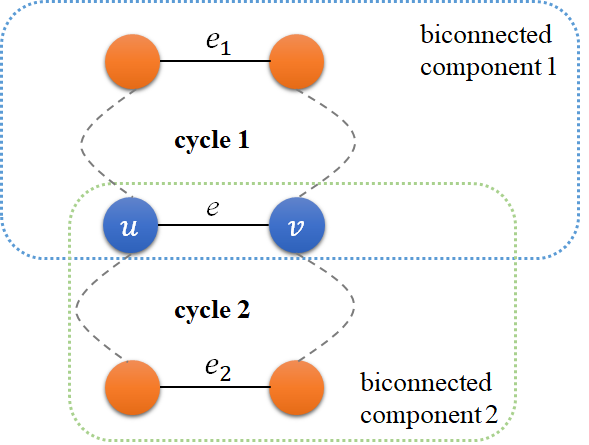
\includegraphics[width=2.5in]{figures/prob2-3-1.png}\\
              \caption{Edge $e_1$ and edge $e_2$ are in biconnected components $G_1$ and $G_2$ respectively}\label{fig2-5}
            \end{figure}
        \item If edge $e_1$ and edge $e_2$ are in $G_1$ and $G_2$ respectively, then without loss of generality, we assume $e_1$ is in $G_1$ and $e_2$ is in $G_2$. Then $e_1$ and $e$ must lie on a common simple cycle since $G_1$ is a biconnected component; similarly, $e_2$ and $e$ must lie on a common simple cycle since $G_2$ is a biconnected component (Fig.~\ref{fig2-5}). Thus, we can form a cycle $C$ including $e_1$ and $e_2$ and it is always possible to \underline{eliminate} \underline{extra nodes and edges in $C$ to form a simple cycle} $C' \subseteq C$ including $e_1$ and $e_2$. Therefore, edge $e_1$ and $e_2$ lie on a common simple cycle.
        \end{itemize}
        In summary, we are able to form a new biconnected component $G_1 \cup G_2$, which is larger than both $G_1$ and $G_2$. And that contradicts the maximality of biconnected components. Therefore, two biconnected components cannot share a same edge $e$.
    \item \textbf{Point 2: } A non-bridge edge $e$ must lie on at least one simple cycle $C$ in $G$ according to the conclusion of sub-question $2$. Therefore, it must be in a biconnected component, since \underline{at least the simple cycle $C$ can be a biconnected components} if it does not have any extra nodes and edges to form a larger one.
    \end{itemize}
    In conclusion, with the two points proved above, we are able to derive the final conclusion: the biconnected components of $G$ partition the nonbridge edges of $G$.
    \end{enumerate}
    \end{proof}
    \clearpage

    \item
    Suppose $G=(V, E)$ is a \textbf{Directed Acyclic Graph} (DAG) with positive weights $w(u, v)$ on each edge. Let $s$ be a vertex of $G$ with no incoming edges and assume that every other node is reachable from $s$ through some path.

    \begin{enumerate}
    	\item
    	Give an $O(|V|+|E|)$-time algorithm to compute the shortest paths from $s$ to all the other vertices in $G$. Note that this is faster than Dijkstra's algorithm in general.
    	\item
    	Give an efficient algorithm to compute the longest paths from $s$ to all the other vertices.
    \end{enumerate}
    \begin{solution} Here are the solutions to each sub-question.
    \begin{enumerate}
    \item Let $d(u)$ denote the length of shortest path from $s$ to $u$, and let a edge set $P(u)$ denote the shortest path from $s$ to $u$. Our algorithm is described as follows.
        \begin{itemize}
        \item Use \textbf{Topological Sort} to order the vertices such that every edge goes from a small vertex to a larger one. It is feasible because the graph is a DAG;
        \item Set $d(s)$ to $0$, and set $P(s)$ to $\varnothing$;
        \item Consider each vertex except $s$ in topological order. Suppose the current vertex is $u$. Since every edge goes from a small vertex to a larger one, the start point $v$ of edge $e = (v, u)$ whose destination is $u$ must be considered before $u$. Therefore, if $P(v) \cup \{(v, u)\}$ forms a shorter path from $s$ to $u$, then update $d(u)$ to $d(v) + w(v, u)$ and update $P(u)$ to $P(v) \cup \{(v, u)\}$;
        \item After considering all vertices in topological order, $d(u)$ will be the length of shortest path from $s$ to $u$, and $P(u)$ will be the specific shortest path.
        \end{itemize}
        The pseudo-code of the algorithm is as follows (Alg.~\ref{alg1}).

        \begin{minipage}[t]{0.8\textwidth}
        \begin{algorithm}[H]
            \KwIn{The Graph $G = (V, E)$ and the weight $w(u, v)$ of every edge $(u, v)$}
            \KwOut{The shortest path $P(u)$ from $s$ to every other vertex $u$ in $G$, and the length $d(u)$ of the shortest path $P(u)$.}

            \BlankLine
            \caption{Compute the single source shortest path in DAG}
            \label{alg1}

            Use \underline{Topological Sort} to order the vertices such that every edge goes from a small vertex to a larger one. Suppose the order is $\{v_0, v_1, \cdots, v_{n-1}\}$.

            $s \leftarrow v_0$ \tcp*[r]{\color{purple}$s$ must be the first vertex of topological order.}

            $d(s) \leftarrow 0$; $P(s) \leftarrow \varnothing$;

            \For{$i \leftarrow 1$ \textbf{to} $n - 1$} {
                $d(v_i) \leftarrow +\infty$;

                \ForEach{edge $(u, v_i) \in G$} {
                    \If{$d(u) + w(u, v_i) < d(v_i)$} {
                        $d(v_i) \leftarrow d(u) + w(u, v_i)$;

                        $P(v_i) \leftarrow P(u) \cup \{ (u, v_i) \}$;
                    }
                }
            }
            \Return{$P(\cdot), d(\cdot)$};
        \end{algorithm}
        \end{minipage}

        \textbf{Correctness Explanation: } The property of DAG can give us a topological order, in which every edge goes from a small vertex to a larger one. This order gives us an optimal structure and we can use it to perform \underline{Dynamic Programming} to compute the shortest paths. Consider the last edge in the shortest path to vertex $v$, it must be $(u, v)$ for some $u$. Thus if we take all possible $u$ into consideration, then the result is bound to be optimal. Since we consider each vertex in topological order, all the starting points are considered before the current vertex $v$, which indicates that their shortest path is already known. Thus, we can use the shortest path to $u$ and edge $(u, v)$ to form a relative-short path from $s$ to $v$. Therefore, the optimal structure is:
        \begin{displaymath}
        d(v) = \left\{
        \begin{aligned}
            & 0 && \quad (v = s) \\
            & \min_{(u, v) \in E}\{d(u) + w(u, v)\} && \quad (v \in V \setminus \{s\})
        \end{aligned}
        \right.
        \end{displaymath}
        The optimal structure is exactly the same as the update strategy in our algorithm.

        Therefore, our algorithm can take every situation into consideration, which indicates that it is correct.

        \textbf{Complexity Explanation: } The time complexity of Topological Sort is $O(|V| + |E|)$ using Topological Sort Algorithm. The main process of our algorithm will consider every vertex $v$ and every edge $(u, v)$ exactly once, therefore, its time complexity is also $O(|V| + |E|)$. Therefore, the total time complexity of our algorithm is $O(|V| + |E|)$.
    \item The algorithm is very similar to algorithm in previous sub-question. We just need to replace all the \texttt{min} to \texttt{max} since we want to compute the longest path. Let $d(u)$ denote the length of longest path from $s$ to $u$, and let a edge set $P(u)$ denote the longest path from $s$ to $u$.

        We only provide the pseudo-code of the algorithm here.

        \begin{minipage}[t]{0.8\textwidth}
        \begin{algorithm}[H]
            \KwIn{The Graph $G = (V, E)$ and the weight $w(u, v)$ of every edge $(u, v)$}
            \KwOut{The longest path $P(u)$ from $s$ to every other vertex $u$ in $G$, and the length $d(u)$ of the longest path $P(u)$.}

            \BlankLine
            \caption{Compute the single source longest path in DAG}
            \label{alg1}

            Use \underline{Topological Sort} to order the vertices such that every edge goes from a small vertex to a larger one. Suppose the order is $\{v_0, v_1, \cdots, v_{n-1}\}$.

            $s \leftarrow v_0$ \tcp*[r]{\color{purple}$s$ must be the first vertex of topological order.}

            $d(s) \leftarrow 0$; $P(s) \leftarrow \varnothing$;

            \For{$i \leftarrow 1$ \textbf{to} $n - 1$} {
                $d(v_i) \leftarrow -\infty$;

                \ForEach{edge $(u, v_i) \in G$} {
                    \If{$d(u) + w(u, v_i) > d(v_i)$} {
                        $d(v_i) \leftarrow d(u) + w(u, v_i)$;

                        $P(v_i) \leftarrow P(u) \cup \{ (u, v_i) \}$;
                    }
                }
            }
            \Return{$P(\cdot), d(\cdot)$};
        \end{algorithm}
        \end{minipage}

        The correctness explanation and complexity explanation are similar to that in the previous sub-question. The time complexity of the algorithm is $O(|V| + |E|)$, which is sufficient enough for graph algorithms.
    \end{enumerate}
    \end{solution}

\end{enumerate}

\vspace{20pt}

\textbf{Remark:} You need to include your .pdf and .tex files in your uploaded .rar or .zip file.

%========================================================================
\end{document}
